%
% ─── CAPITULO 7: INTRODUCCION AL RAY TRACING ────────────────────────────────────
%

En los anteriores capítulos hemos visto cómo asignar colores a los píxeles utilizando el fragment shader y cómo dibujar hermosos fractales en la superficie que ocupan dos triángulos. Sin embargo, no hemos podido movernos de las dos dimensiones. Esto se debe a la dificultad que de por sí supone que en 2D un píxel puede representar un único punto del plano mientras que en 3D un píxel representa infinitos puntos del espacio. Nuestro objetivo ahora es poder visualizar escenas simples en 3D para posteriormente renderizar fractales en 3D.

\section{Definición de Ray-Tracing}

En el mundo de la informática gráfica existen dos formas fundamentales de proceder al renderizado de escenas. Supongamos que tenemos una escena 3D con varios objetos, como pueden ser por ejemplo un cubo y un par de esferas y queremos visualizar la misma en un canvas 2D.
\begin{itemize}
    \item Una de las formas de renderizarlo es identificar para cada objeto (también llamado primitiva) qué píxeles ocupan y asignar color a cada píxel, aplicando posibles modelos de iluminación y texturas. Esta es la técnica conocida como \textbf{rasterización}.
    \item Otra forma es, para cada pixel, calcular qué primitivas ocupan posiciones del espacio asociadas a dicho píxel y colorearlo dependiendo de la primitiva más cercana al observador. Esta es la base del \textbf{Ray-Tracing}.
\end{itemize}

Más en profundidad, la idea es situar al espectador en una cierta posición de la escena y colocar frente a él un plano, el cual estará dividido en tantos píxeles como tenga el canvas, de tal manera que se `trazan rayos' que salen desde la posición del espectador en dirección a cada píxel, por lo que se lanzan tantos rayos como píxeles haya. El rayo atraviesa el plano y avanza por la escena hasta que encuentra la intersección con un objeto. En este caso, se calcula en qué punto se ha alcanzado la intersección y se evalúa un modelo de iluminación o se asigna un color dependiendo de las características de la escena. también es posible que el rayo no alcance ningún objeto y se pierda, en cuyo caso habría que saber qué hacer con los píxeles cuyos rayos se pierden en el infinito. En la imagen \ref{fig:RT} se puede observar un esquema aclarativo del funcionamiento de este método.

\begin{figure} [ht]
    \centering
    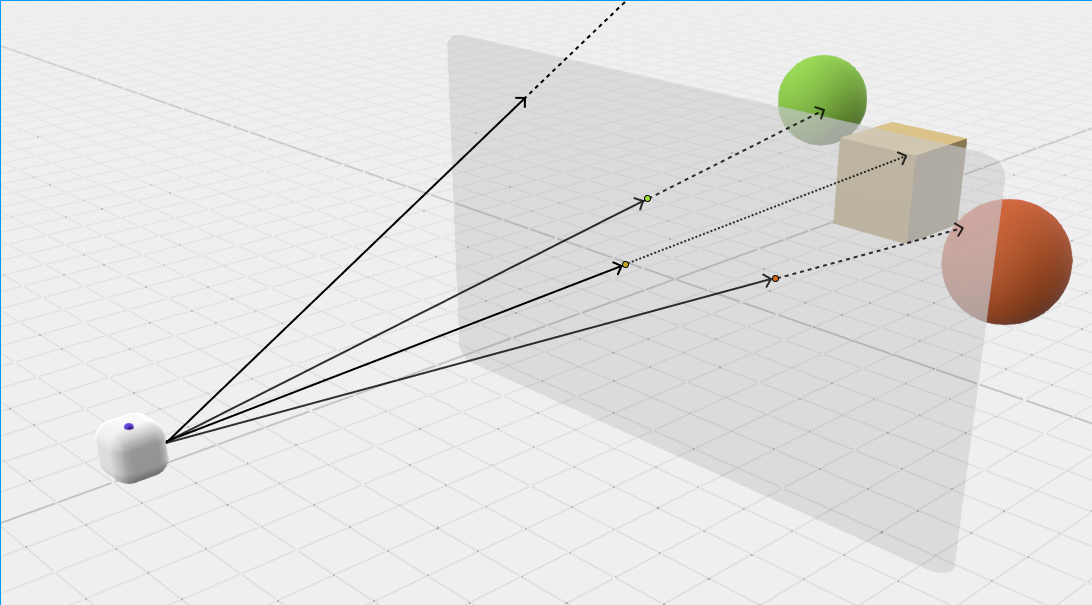
\includegraphics[scale = 0.35]{img/C7/RT.png}
    \caption{Esquema básico del funcionamiento del Ray-Tracing}
    \label{fig:RT}
\end{figure}

La principal ventaja que tiene el Ray-Tracing (en adelante RT) sobre la rasterización es que este trazado de rayos nos permite facilitar el cálculo de los reflejos y sombras creados por las iluminaciones del entorno, consiguiendo así efectos mucho más realistas en las escenas. Además, recordemos que las figuras fractales que perseguimos no es posible dibujarlas mediante un conjunto de vértices o aristas al no ser objetos de la geometría euclídea, por lo que sería muy difícil expresarlos como primitivas rasterizables. Lo más natural es lanzar rayos y, en caso de detectar intersección con el fractal estimar la normal en dicho punto y aplicar un modelo de iluminación. Es por esta serie de razones por las que para nuestro objetivo necesitamos programar un \textit{ray-tracer} inicialmente básico con el objetivo futuro de renderizar fractales 3D.

Sin embargo, este algoritmo tiene una principal desventaja, y es que es un proceso muy costoso, y más aún cuanto más detalle queramos conseguir. Es por esto que ha sido muy difícil dar el salto al ray tracing en tiempo real. Por ejemplo, en el mundo de los videojuegos, NVIDIA, que es una famosa empresa desarrolladora de tarjetas gráficas, comenzó a desarrollar algoritmos para poder utilizar RT en sus tarjetas hace varios años, pero hasta finales de 2018 no salieron las primeras gráficas con estas características al mercado. Por su parte, los juegos también deben soportar el algoritmo, por lo que aún son una minoría de videojuegos los que en la actualidad soportan Ray Tracing. En un futuro no muy lejano es posible que haya una tendencia a un desarrollo masivo de juegos que utilicen RT, pero de momento solo tenemos algunos ejemplos como Battlefield V, Minecraft, Metro Exodus, Watch Dogs y Call of Duty: Modern Warfare (2019).

Sin embargo, a pesar de dicha desventaja veremos que nuestro código puede ejecutarse en tiempo real, teniendo en cuenta siempre que debemos evitar el uso de funciones que comprometan la velocidad de ejecución. Por ejemplo, la función \verb|pow| es muy lenta, por lo que debemos evitar usarla cuando se usen potencias enteras.

En este caso, y de manera similar a la efectuada con los fractales 2D, el vertex shader utilizado es trivial, de hecho es exactamente el mismo que se puede encontrar al inicio del capítulo \ref{chap:fractales-2D}. Por tanto el grueso de la programación se hará de nuevo en el fragment shader, que es el que se ejecuta una vez por píxel. Por su parte, usaremos JavaScript para pasarle variables uniform al shader y para añadir interactividad a la escena. Las siguientes secciones irán dedicadas a explicar la programación del fragment shader.

\section{Creación del rayo}

Recordamos que cuando se trataba de fractales 2D utilizamos una transformación lineal para identificar cada píxel con un punto del plano complejo (inicio de la sección \ref{section:fs-2D}). En este caso debemos identificar cada píxel con un punto no del plano complejo, sino del que llamaremos \textit{plano de proyección}, que es el plano que colocamos frente al espectador dividido en tantos píxeles como tenga el canvas, de forma que se trazan rayos desde el espectador y hacia dicho píxel. En este caso utilizamos un canvas de $1280\times 720$ píxeles, que guarda una proporción de $16:9$, que es de hecho la más habitual.
\begin{lstlisting}
<canvas id="glCanvas"  width="1280" height="720"></canvas>
\end{lstlisting}

Inicialmente, supongamos que el observador se sitúa en el punto $(0,0,0)$ y que el plano de proyección se sitúa a distancia 1 en el eje negativo $Z$. Esta distancia del observador al plano de proyección es la conocida como la \textit{distancia focal}. Se denomina \textit{lookfrom} al punto desde el que observa (en el que se sitúa) el observador y \textit{lookat} al punto hacia el que mira, que en este caso sería el $(0,0,-1)$. 

Como convención asumimos que a la derecha se sitúa el eje positivo $X$, hacia arriba el eje positivo $Y$ y el `interior de la pantalla' es el eje negativo $Z$. Asumimos ahora también que el plano de proyección tiene 2 unidades de alto, lo cual implica que si el ratio ancho/alto es $16/9$ entonces el ancho es de $3.55$ unidades, aunque ese es un valor que calcularemos y almacenaremos en una variable y no importará realmente cual sea.

Un rayo es en realidad simplemente una semirrecta de $\R^3$, las cuales están unívocamente determinadas por un punto $p$ del espacio afín $\R^3$ al cual llamaremos \textit{origen} y por un vector $v$ del espacio vectorial $\R^3$ que denominamos \textit{dirección}. De esta forma, un rayo puede ser expresado como la imagen de la función

$$
R(t) = p + t\cdot v \ \ \forall t\in\R_0^+,
$$
de forma que para cualquier punto $p_0$ del rayo $R$ existe un único $t_0\in\R_0^+$ tal que $R(t_0) = p_0$.

A nivel de código GLSL, la manera de representar un rayo será utilizando una estructura (\verb|struct|) que denominaremos \verb|Ray|. Las estructuras en GLSL son muy parecidas en sintaxis y también en uso a las del lenguaje C. 

\begin{lstlisting}
struct Ray {
    vec3 orig;      // Ray's origin
    vec3 dir;       // Ray's direction
};
\end{lstlisting}

Y si dado un rayo $R$ queremos calcular qué punto de $\R^3$ le corresponde a cierto $t\in\R_0^+$, utilizamos la siguiente función.

\begin{lstlisting}
vec3 ray_at(Ray R, float t){
    return R.orig + t*R.dir;
}
\end{lstlisting}

Esta función nos será útil a la hora de calcular el punto exacto en el que se produce una intersección rayo-objeto cuando solo se conoce la distancia $t$ a la que se produce el impacto.

\begin{observacion}
    Realmente se pueden utilizar valores de $t\in\R$ positivos o negativos, pero pensemos que los valores negativos corresponden a puntos del rayo situados detrás del observador, que no se pueden ver, por lo que es preferible restringirnos a valores no negativos.
\end{observacion}

Una vez tenemos determinada una forma de representar un rayo, es momento de crear un rayo cuyo origen sea la posición del observador y su dirección sea el vector que tiene como origen el observador y como destino el punto del plano de proyección que identificamos con el píxel. En la situación hipotética que hemos planteado antes en la cual $lookfrom=(0,0,0)$, llamamos $df$ a la distancia focal, $PP_{height}=2$ a la altura del plano de proyección, $PP_{width}$ a la anchura del plano de proyección, $AR = 16/9$ (\textit{aspect ratio}) a la proporción $AR = \frac{PP_{width}}{PP_{height}}$, de forma que se verifica $PP_{width}=AR\cdot PP_{height}$. Con estas variables, llamemos $LLC$ (\textit{Lower Left Corner}) al punto situado en la esquina inferior izquierda del plano de proyección, entonces:
$$
LLC = lookfrom - PP_{width}\cdot(1,0,0) - PP_{height}\cdot(0,1,0) - df \cdot (0,0,1)
$$

Una vez conocemos la esquina superior izquierda, la cual identificamos con el píxel inferior izquierdo del canvas, debemos recuperar la transformación \ref{eq:transformacion-lineal-3}, pero en este caso nos debemos llevar la región $[0,1280]\times[0,720]$ a $[0,PP_{width}]\times[0,PP_{height}]$. La transformación por tanto en este caso es

\begin{equation}
    \label{eq:transformacion-lineal-4}
    \begin{split}
        \phi : [0,1280]\times [0,720] & \longrightarrow [0,PP_{width}]\times[0,PP_{height}] \\
        (x,y) & \longmapsto \left(\frac{PP_{width}\cdot x}{1280},\frac{PP_{height}\cdot y}{720}\right)
    \end{split}
\end{equation}
donde $(x,y)$ son las coordenadas de dispositivo en términos de píxeles a las que puede acceder el fragment shader a traves de \verb|gl_FragCoor|. Y así identificamos el alto y ancho del canvas con el alto y ancho del plano de proyección, de manera que a partir de estos valores y conociendo qué punto se sitúa en la esquina inferior izquierda podemos definitivamente calcular con qué punto del plano de proyección identificamos el píxel:
$$
destiny := LLC + \phi(x,y)
$$
Y por tanto, la dirección del rayo sería
$$
v = LLC + \phi(x,y) - lookfrom
$$
y el origen sería obviamente el punto $lookfrom$.

El código GLSL que hemos utilizado hasta este punto sería el siguiente:

\begin{lstlisting}

Ray get_ray(vec3 lookfrom, vec3 lookat, 
    float viewport_width, float viewport_height, 
    float u, float v) {
    
    Ray R;
    R.orig = lookfrom;
    float df = length(lookat - lookfrom); // Distancia focal
    vec3 lower_left_corner = lookfrom
        - viewport_width/float(2.0)*vec3(1.0, 0.0, 0.0)
        - viewport_height/float(2.0)*vec3(0.0, 1.0, 0.0) 
        - df*vec3(0.0, 0.0, 1.0);
    R.dir = lower_left_corner 
        + u*viewport_width 
        + v*viewport_height 
        - lookfrom;
    return R;
}

// ... 

// Dimensiones del canvas
float aspect_ratio = float(16.0) / float(9.0);
float image_width = 1280.0;
float image_height = image_width / aspect_ratio;

vec2 uv = gl_FragCoord.xy / vec2(image_width, image_height); // Coordenadas de dispositivo normalizadas [0,1]
float u = uv.x;
float v = uv.y;

// Dimensiones del plano de proyeccion
float viewport_height = float(2.0);
float viewport_width = viewport_height * aspect_ratio;

// lookfrom y lookat
vec3 lookfrom = vec3(0.0, 0.0, 0.0);
vec3 lookat = vec3(0.0, 0.0, -1.0);

// Ray
Ray R = get_ray(lookfrom, lookat, 
    viewport_width, viewport_height, 
    u, v);
\end{lstlisting}

Y de esta forma el fragment shader obtiene un rayo por cada píxel que tiene como origen la posición del observador y que interseca con el punto correspondiente al píxel en el plano de proyección.

\section{El background}

Una vez tenemos creado el rayo asignado a un píxel debemos asignar un color. La función que dado un rayo $R$ devuelve el color del cual colorearemos el píxel la llamaremos \verb|ray_color|. Esta función se verá sometida a muchos cambios, sobre todo en sus argumentos dependiendo de los elementos que compongan la escena, pero de momento asumimos una escena vacía. Que la escena esté vacía supone que ningún rayo interseca ninguna superficie, pero independientemente de ello hay que asignar un color al píxel. Esta asignación de color a un rayo que no interseca ninguna superficie determina el fondo (\textit{background}) de la escena, y esta decisión que tomaremos ahora sobre cómo colorear el fondo nos acompañará durante el resto del proyecto. 

En concreto, hemos decidido simular algo parecido al cielo mediante un degradado vertical de un \textcolor{background-blue}{azul} \verb|rgb(127, 178, 255)| a blanco \verb|rgb(255, 255, 255)|, definiendo el color a partir de la componente $y$ del vector director normalizado. Mostramos el código correspondiente también para clarificar esta descripción.

\begin{lstlisting}
vec4 ray_color(Ray R) {
    // R does not hit any surface
    vec3 unit_direction = normalize(R.dir);
    float t = 0.5*(unit_direction.y + 1.0);
    return vec4((1.0-t)*vec3(1.0,1.0,1.0) + t*vec3(0.5,0.7,1.0), 1.0);
}
\end{lstlisting}

De esta forma, si el rayo apunta hacia arriba el color del píxel será más azul y si apunta hacia abajo más blanco. En la imagen \ref{fig:background} podemos ver el gradiente utilizado.

\begin{figure} [ht]
    \centering
    
\includegraphics[scale = 0.35]{img/C7/background-gradient.png}
    \caption{Gradiente utilizado para el fondo de la escena}
    \label{fig:background}
\end{figure}

Y en la imagen \ref{fig:first-render} podemos ver el resultado de efectuar la llamada a \verb|ray_color| una vez creado el rayo. Esta es la primera escena 3D renderizada utilizando RT en WebGL. Nótese que en la imagen no aparecen todos los colores del gradiente de la imagen \ref{fig:background}, y esto se debe a que los rayos que se trazan en esta situación inicial no cubren todas las alturas posibles. Por ejemplo, no se traza un rayo totalmente vertical hacia arriba ni hacia abajo, solo se trazan las alturas necesarias para cubrir el plano de proyección. Esto nos da una manera de orientarnos en la altura una vez parametricemos la posición y orientación de la cámara, de tal manera que si vemos el fondo muy azul podemos asumir que se está mirando `al cielo' y si el color es blanco se estará mirando `al vacío'. 

\begin{lstlisting}
gl_FragColor = ray_color(R);
\end{lstlisting}

\begin{figure} [ht]
    \centering
    
\includegraphics[scale = 0.35]{img/C7/first-render.png}
    \caption{Primera escena vacía renderizada}
    \label{fig:first-render}
\end{figure}

\section{Visualizando una escena sencilla}

Hasta este momento hemos diseñado la estructura del ray tracer como un observador situado en la posición $(0, 0,0)$ y proyectando una escena vacía en un plano de $2$ unidades de alto y guardando un ratio de 16:9. Sin embargo, aún queda lo más importante, que es añadir cuerpos a la escena con los que los rayos puedan intersecar. El objetivo de esta sección es describir la metodología y el código GLSL necesario para dibujar una escena con una o varias esferas y un plano con textura de tablero de ajedrez.

\subsection{Renderizando una esfera}

Primero introduciremos código para visualizar una esfera. Por simple geometría euclídea sabemos que, fijado un centro $c=(c_x,c_y,c_z)\in\R^3$ y un radio $r\in\R^+$, una esfera $S$ se define como aquellos puntos de $\R^3$ tales que su distancia a $c$ es $r$, es decir:
$$
S = \{p\in\R^3:\|p-c\|=r\} = \{p\in\R^3:(p-c)\cdot (p-c)=r^2\}. 
$$
donde en esta definición el operador $\cdot$ denota el producto escalar de dos vectores. Si recordamos que los puntos que componen un rayo $R$ se pueden expresar como $R(t)= p_0 + vt$ (donde $p_0$ es el origen del rayo y el vector $v$ su dirección) con valores de $t$ reales no negativos, podemos calcular la intersección rayo-esfera sin más que resolviendo la ecuación
$$
(R(t)-c)\cdot(R(t)-c)=r^2
$$
de tal manera que, si resolvemos la ecuación en $t$ podremos saber en qué valor de $t$ golpea el rayo la esfera, si es que efectivamente lo interseca.
\begin{eqnarray*}
    (R(t)-c)\cdot(R(t)-c)=r^2 \\
    (p_0 + vt - c)\cdot(p_0 + vt - c) = r^2 \\
    (vt + (p_0 -c))\cdot (vt + (p_0 -c))= r^2 \\
    (v\cdot v)t^2 + 2(v\cdot(p_0-c))t + (p_0 -c)\cdot (p_0 -c) - r^2 = 0 
\end{eqnarray*}
Y esto es una ecuación de segundo grado en $t$. Esto nos dice que el rayo puede intersecar dos veces con la esfera (secante), una única vez si el discriminante se anula (tangente) o ninguna si el discriminante es negativo (el rayo no interseca con la esfera). En caso de que exista intersección debemos quedarnos con el valor de $t$ más pequeño, que es el más cercano a la posición del espectador. También debemos quedarnos únicamente con valores de $t$ positivos, pues si es negativo significa que la esfera está detrás del observador, en cuyo caso no es visible.

A nivel de código podemos codificar una esfera como un \verb|struct| cuyos elementos sean su centro y su radio

\begin{lstlisting}
struct Sphere{
    vec3 center;
    float radius;
};
\end{lstlisting}

Además, para el futuro necesitaremos una estructura que almacene información sobre un impacto rayo-superficie. Información como el punto en el que se produce, en qué $t$, la normal a la superficie en ese punto, etc. En estas fases tan tempranas igual no es tan necesario pero pronto encontraremos su utilidad.

\begin{lstlisting}
struct Hit_record {
    vec3 p;         // Punto donde se produce el impacto
    vec3 normal;    // Normal a la superficie en el punto p
    float t;        // Valor de t para el que el rayo impacta
    bool hit;       // True sii se golpea alguna superficie
};
\end{lstlisting}

Claro que los tres primeros campos solo tendrán sentido si el campo \verb|hit| es verdadero, si es falso no tiene sentido calcular ni consultar los demás. A continuación presentamos el código GLSL para visualizar una esfera utilizando estas estructuras.